\graphicspath{{members/cm/figures/}}

\subsection{Building the foundation of the tomato plants}
\input{members/cm/authors}

The goal of the simulation is to create a variety of different realistic tomato plants. The first step is therefore to determine which parameters describe a realistic tomato plant. A tomato plant can be split in four major parts; stem, leaves, flowers, fruits. Each of which, have their own properties, which can vary from plant to plant in a certain range. For example, if a tomato plant carries ripe fruits these are red, round and have a certain size. But how ripe the fruits are and the health status of the plant, can lead to variations in size and color of the fruits. And the amount and position of the fruits are variable, as well. 

In order to create this variability PlantStudio is used.
PlantStudio is a parameter-driven simulation tool, which can be used for the simulation of various non-woody plants throughout their life cycle.
It provides various parameters concerning the structure and the growth of the plant.
It starts with a collection of questions regarding the optics of the plant, containing information about the stem, leaves, flowers and fruits.
This enables an individual adjustment of color, shape, amount and distribution for each of these plant parts. A detailed descriptions of the settings used in this project can be found in table \ref{tab:parameters_plantStudio}. Thanks to the randomize function provided by PlantStudio a multitude of different plants with these parameters can be created.\\

For each created plant PlantStudio animates a life cycle going from the spearing of the plant to the full-grown tomato plant with ripe fruits. The duration of the life cycle and at which point the fruits start to grow, can be manually adjusted to create a realistic representation. \\

\begin{longtable}[c]{@{}p{0.15\textwidth}p{0.45\textwidth}p{0.4\textwidth}@{}}
	\caption{General parameters set in PlantStudio describing the growth behavior of tomato plants.}
	\label{tab:parameters_plantStudio}\\
	\toprule
	& Description                                                                                                                                                                                                                 & Settings                                                                                                                                                                      \\* \midrule
	\endhead
	%
	\bottomrule
	\endfoot
	%
	\endlastfoot
	%
	Meristems               & Meristems are buds from which leaves and branches grow.                                                                                                                                                                     & \vspace{-25pt}
	 \begin{itemize}
		\item opposing to each other \vspace{-10pt}
		\item medium amount of branches \vspace{-10pt}
		\item secondary branches \vspace{-10pt}
		\item angle stem/branch: medium \vspace{-10pt}   
	\end{itemize} \\
	Internodes              & Internodes are portions of plant stem between leaves and determine how short or tall, straight or viney, and stiff or flexible the plant will be                                                                            & \vspace{-25pt}
	\begin{itemize}
		\item long \vspace{-10pt}
		\item medium thickness \vspace{-10pt}
		\item introduce some curve to the plant \vspace{-10pt}
	\end{itemize} \\
	Leaves                  & Leaves are drawn using a 3D-object. The leaf is drawn bigger as the plant grows. Leaves are connected to the plant by a stalk called petiole& \vspace{-25pt}
	\begin{itemize}
		\item pre-build shape: tomato leaf\vspace{-10pt}
		\item small size \vspace{-10pt}
		\item petiole of medium length \vspace{-10pt}
		\item angle stem/leaf: large \vspace{-10pt}
	\end{itemize} \\
	Compound leaves         & A compound leaf contains $>$=2 leaflets. Leaflets look like small whole leaves, but fit together in the same pattern for all leaves of the plant. A leaf without leaflets is a simple leaf & \vspace{-25pt}
	\begin{itemize}
		\item pinnate leaves (seven leaves are ordered feather like) \vspace{-10pt}
		\item leaflet are in a medium distance to each other \vspace{-10pt}
	\end{itemize} \\
	Inflorescence placement & An inflorescence holds fruits and flowers on a plant. It is divided in apical, which means at the end of the plant stems and axillar, which means between the angles between the stem and the leaf.         & \vspace{-25pt}
	\begin{itemize}
		\item no apical inflorescence \vspace{-10pt}
		\item multiple axillary inforescneces (10)\vspace{-10pt}
		\item primary stems have a medium length\vspace{-10pt}
	\end{itemize} \\
	Inflorescence drawing   & Inflorescence can have a variety of shapes                                                                                                                                                                                  & \vspace{-25pt}
	\begin{itemize}
		\item 10 flowers per inflorescence\vspace{-10pt}
		\item placed in spikes\vspace{-10pt}
		\item stem thickness:  medium\vspace{-10pt}
	\end{itemize} \\
	Flowers                 & Like leaves flowers are drawn as 3D objects, with each 3D object representing one petal of the flower.                                                                                                                      & \vspace{-25pt}
	\begin{itemize}
		\item 4 small, yellow pedals\vspace{-10pt}
		\item pre-built shape: corn leaves\vspace{-10pt}
		\item elongated and pointy\vspace{-10pt}
	\end{itemize} \\
	Fruits   & Fruits are drawn like flowers, but with a portion of fruit rotated around instead of petals                                                                                                                                 & \vspace{-25pt}
	\begin{itemize}
		\item common fruit section 1\vspace{-10pt}
		\item 10 fruit sections per fruit\vspace{-10pt}
		\item huge size\vspace{-10pt}
		\item unripe fruits: green\vspace{-10pt}
		\item ripe fruits: red\vspace{-10pt}
	\end{itemize}
\\* \bottomrule
\end{longtable}


\begin{figure}[ht]
	\centering
	\begin{subfigure}{.24\textwidth}
		\centering
		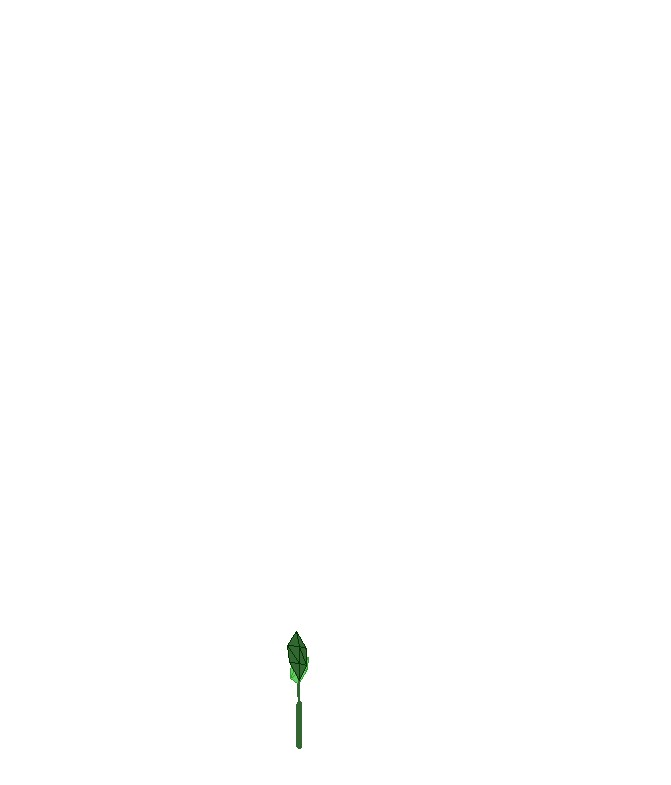
\includegraphics[width=\linewidth]{plantAging001.jpg}
		\label{fig:sub1}
	\end{subfigure}
	\begin{subfigure}{.24\textwidth}
		\centering
		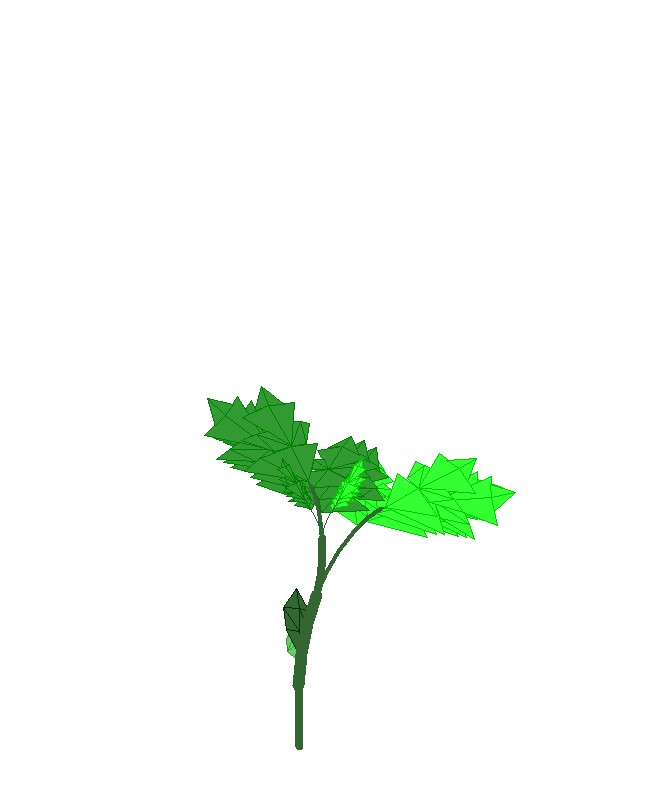
\includegraphics[width=\linewidth]{plantAging002.jpg}
		\label{fig:sub2}
	\end{subfigure}%
	\begin{subfigure}{.24\textwidth}
		\centering
		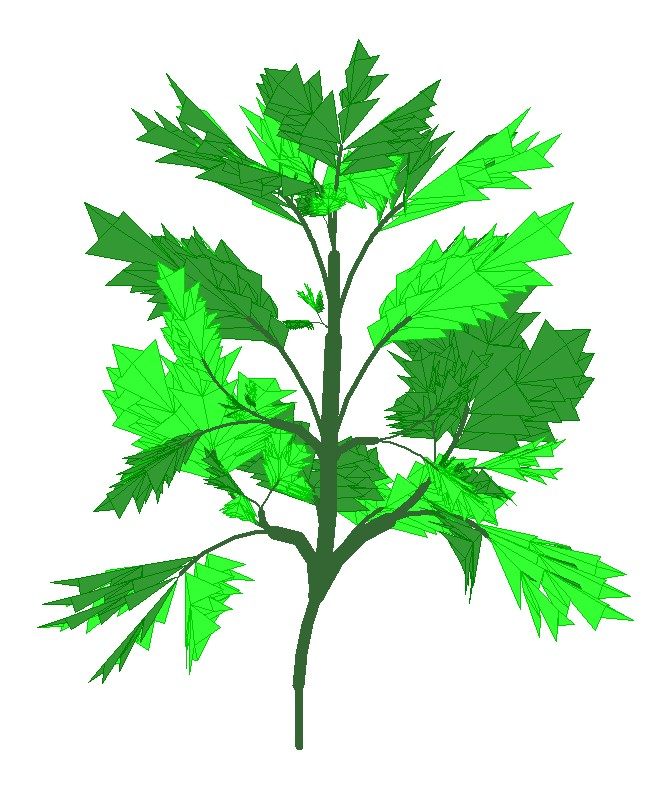
\includegraphics[width=\linewidth]{plantAging003.jpg}
		\label{fig:sub3}
	\end{subfigure}%
	\begin{subfigure}{.24\textwidth}
		\centering
		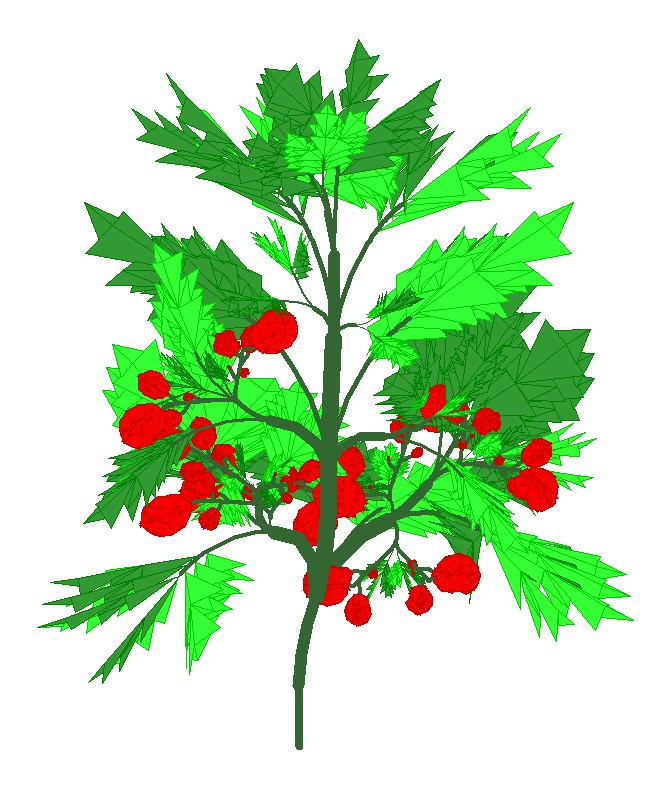
\includegraphics[width=\linewidth]{plantAging004.jpg}
		\label{fig:sub4}
	\end{subfigure}%
	\caption{Example of a tomato plant created with PlantStudios in four different stages of growth}
	\label{fig:plantStudio}
	\vspace{-10pt}
\end{figure} 


The created plants have the general parameters of tomato plant but do not look realistic thus far, which can be seen in figure \ref{fig:plantStudio}. The shortcomings of the simulation, like the missing texture and material, can be solved by using a second simulation tool, like Blender. This is enabled by PlantStuios option to export the plants as wavefronts (.obj). Here, we created a total of 42 different plants, which were saved grouped by individual plant parts, which allows to change each leaf, fruit or flower individually in later steps.



\subsection{Importing and placing plants in Blender}
\input{members/cm/authors}
\begin{wrapfigure}{r}{0.5\textwidth} 
	\vspace{-25pt}
	\begin{center}
		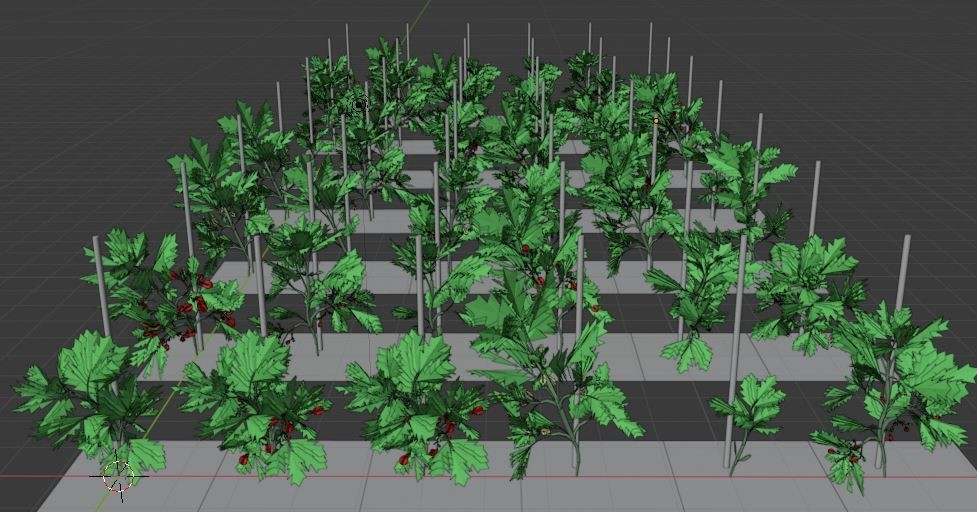
\includegraphics[width=0.45\textwidth]{BlenderImport.JPG}
		\caption{Import of 42 randomly selected plants into Blender with 6 plants per row and soil and pole for each plant.}
		\label{fig:BlenderImport}
	\end{center}
	\vspace{-20pt}
	\vspace{1pt}
\end{wrapfigure} 

The tomato plant can be imported into Blender. Blender is an open source computer graphics software, which can be used for visual effects, 3D models, etc. The purpose of using Blender is to import the in PlantStudio created plants and  add details, shading, rendering and lighting. The script written to import the plants can be easily adjusted in the number of plants that should be planted and the number of plants that are planted in each row. Which plants are planted is randomly selected from the 42 plants exported from PlantStudio.

\lstinputlisting[language=Python, linerange={12-14}, frame=single, caption = Given a folder \textit{directory\_im} containing obj files a specific number of plants are randomly selected ]{members/cm/import_plants.py}\vspace{5pt}


The plants are than imported and placed in multiple rows of a specific length, that can be set by the user. Here, it is important to select to split the geometry by group, in order to individually adjust each leaf or fruit section. In order to be able to differentiate between the various plants, each plant is placed in its own collection. 

\lstinputlisting[language=Python, linerange={21-39}, frame=single, caption = Inorder to place the plants like they would be placed in the greenhouse we need to know how many plants should be planted and how many fit in one row.]{members/cm/import_plants.py}\vspace{5pt}

Each plant is positioned next to a pole to fix it and on a square of soil. In this step we add these features without any texture and material. These will be added at a later point to further increase the closeness to reality. 

\lstinputlisting[language=Python, linerange={43-49}, frame=single, caption = Placement of the pole next to each plant. Placement of soil is don analog]{members/cm/import_plants.py}\vspace{5pt}

